\documentclass{article}
\usepackage{graphicx} % Load the graphicx package  

% Define a style for Python code
\begin{document}

\title{Exercício 5} 
\author{Arthur Felipe Reis Souza}
\date{\today}
\maketitle

\section{Introduction}
O exercício consiste em aplicar as rede neurais do tipo ELM para resolver problemas multidimensionais. Serão utilizados 2 conjunto de dados, o conjunto de dados Breast Cancer e o conjunto de dados Statlog.
\vspace{20pt}

\subsection{Breast Cancer}
O dataset Breast Cancer foi utilizado.

\begin{center}

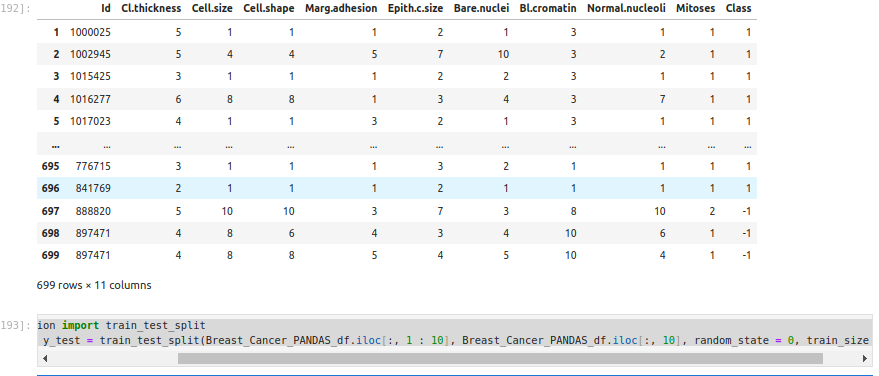
\includegraphics[height=2in]{Ex6/Breast_Cancer/Plot_Breast.png}

\end{center}

\vspace{10pt}
Inicialmente foi utilizado uma rede ELM com 5 neurônios na camada intermediária. Com apenas 5 neurônios na camada intermediária, é possível concluir que o modelo obteve um alto erro para os dados tanto de treino quanto de teste, os erros foram bastante altos e podemos considerar isso como um underfitting. A matriz de confusão e o gráfico de separação estão plotados abaixo :

\begin{center}

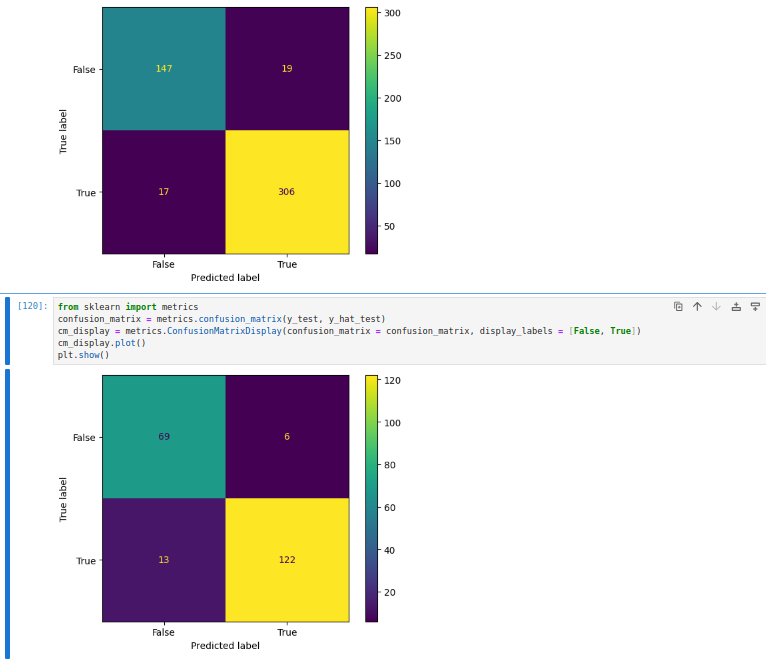
\includegraphics[height=3in]{Ex6/Breast_Cancer/matrix_conf_5.png}
\vspace{10pt}

\end{center}

\begin{center}

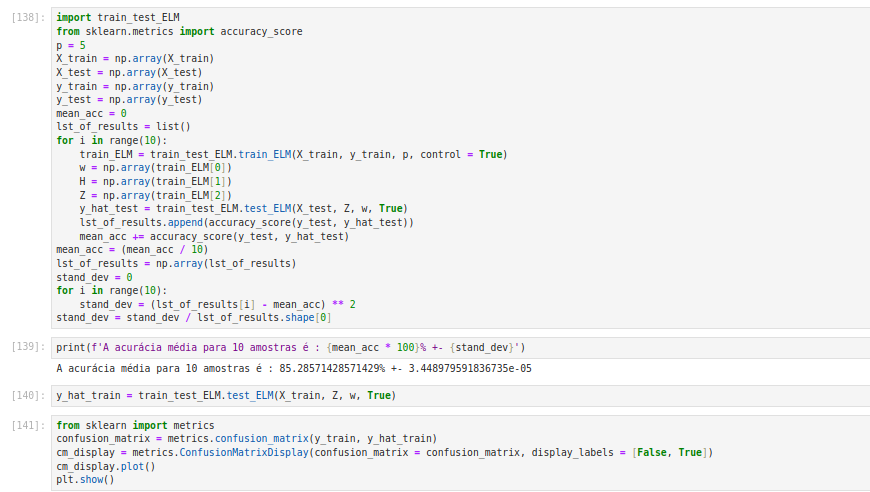
\includegraphics[height=3in]{Ex6/Breast_Cancer/acc_5.png}
\vspace{10pt}

\end{center}

\vspace{5pt}
Utilizando com 10 neuronios obtemos os resultados : 

\begin{center}

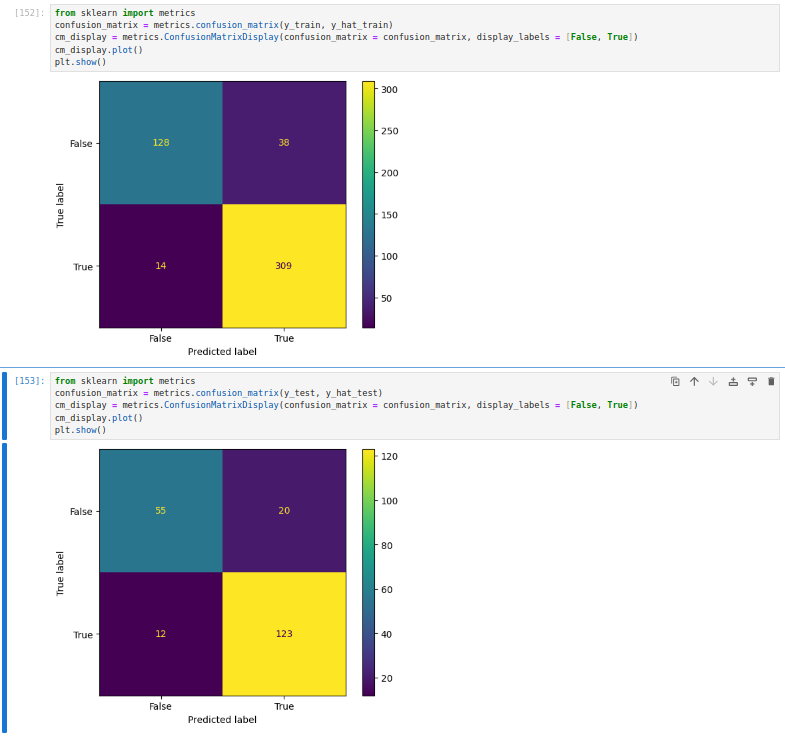
\includegraphics[height=3in]{Ex6/Breast_Cancer/conf_matrix_10.png}
\vspace{10pt}

\end{center}

\begin{center}

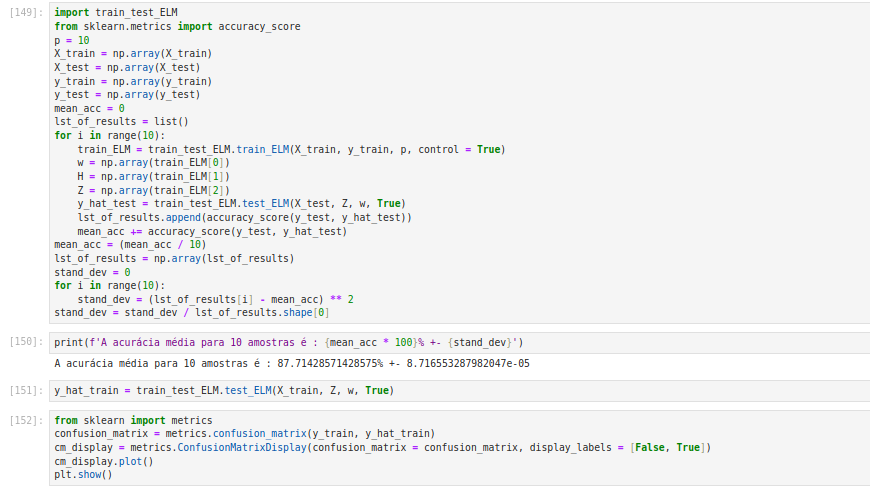
\includegraphics[height=3in]{Ex6/Breast_Cancer/acc_10.png}
\vspace{10pt}

\end{centerw}

\vspace{5pt}
Utilizando com 30 neuronios obtemos os resultados : 

\begin{center}

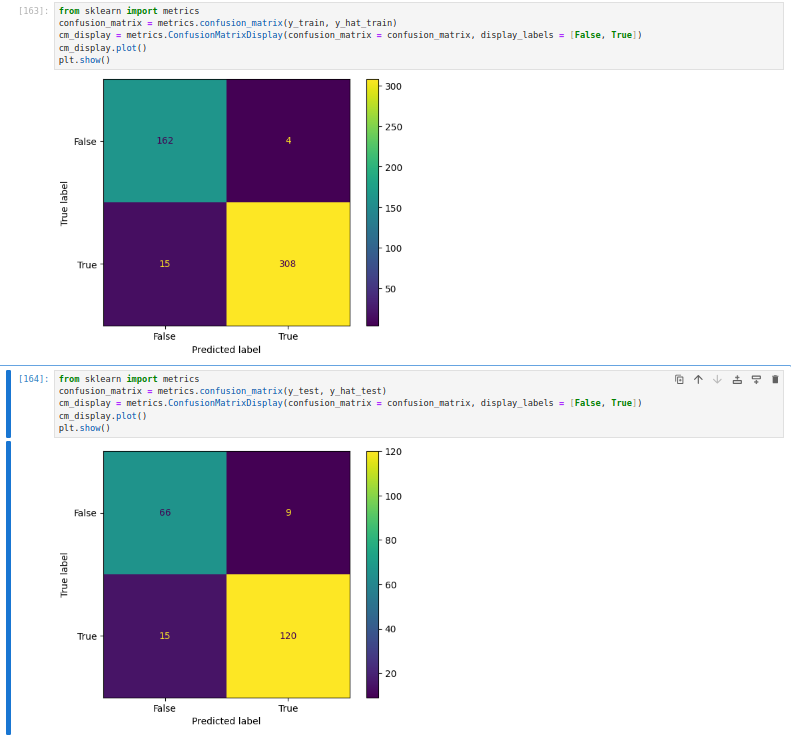
\includegraphics[height=3in]{Ex6/Breast_Cancer/matrix_conf_30.png}
\vspace{10pt}

\end{center}

\begin{center}

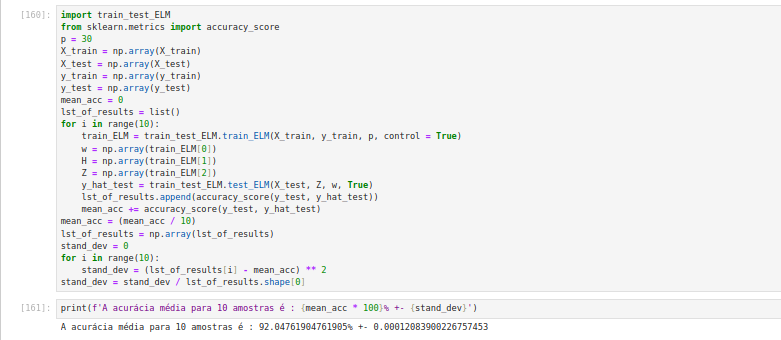
\includegraphics[height=3in]{Ex6/Breast_Cancer/acc_30.png}
\vspace{10pt}

\end{center}

\vspace{5pt}
Utilizando com 50 neuronios obtemos os resultados : 

\begin{center}

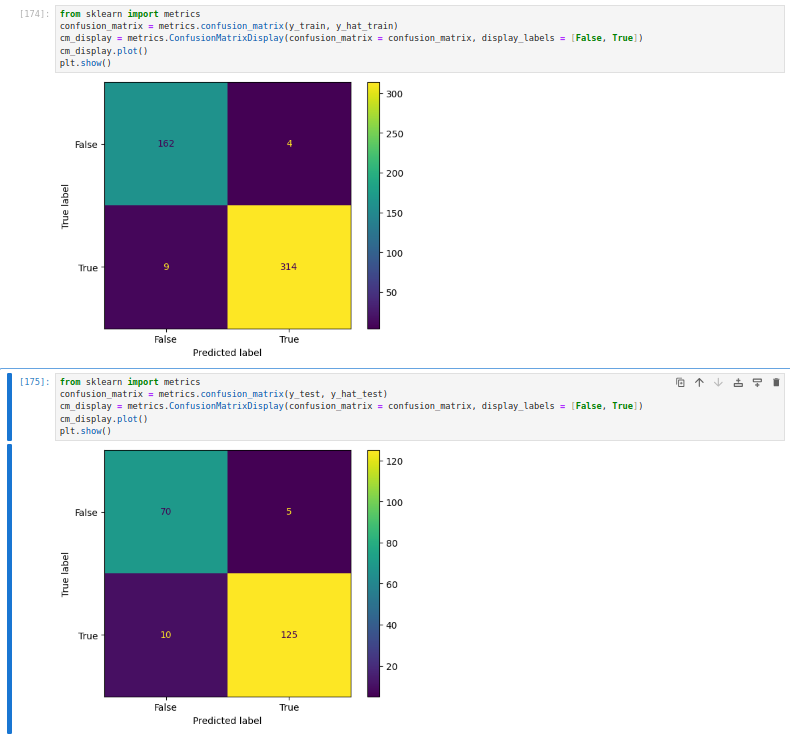
\includegraphics[height=3in]{Ex6/Breast_Cancer/matrix_conf_50.png}
\vspace{10pt}

\end{center}

\begin{center}

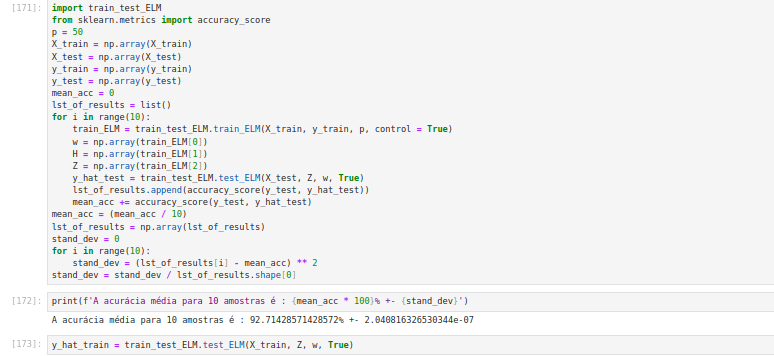
\includegraphics[height=3in]{Ex6/Breast_Cancer/acc_50.png}
\vspace{10pt}

\end{center}



\vspace{5pt}
Utilizando com 100 neuronios obtemos os resultados : 

\begin{center}

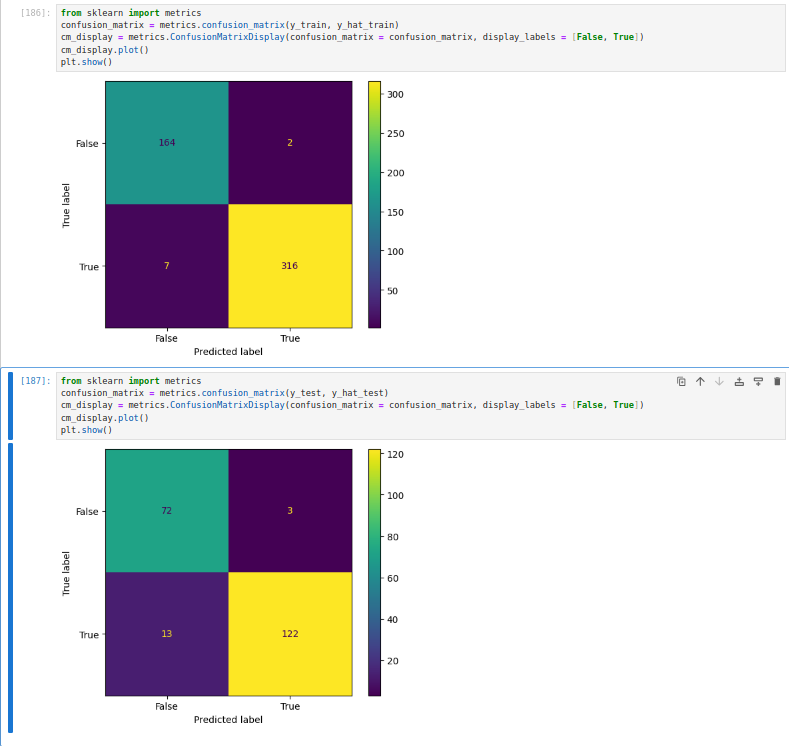
\includegraphics[height=3in]{Ex6/Breast_Cancer/matrix_conf_100.png}
\vspace{10pt}

\end{center}

\begin{center}

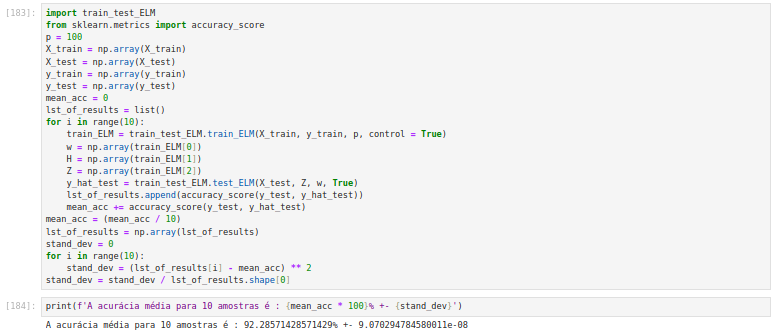
\includegraphics[height=3in]{Ex6/Breast_Cancer/acc_100.png}
\vspace{10pt}

\end{center}



\vspace{5pt}
Utilizando com 300 neuronios obtemos os resultados : 

\begin{center}

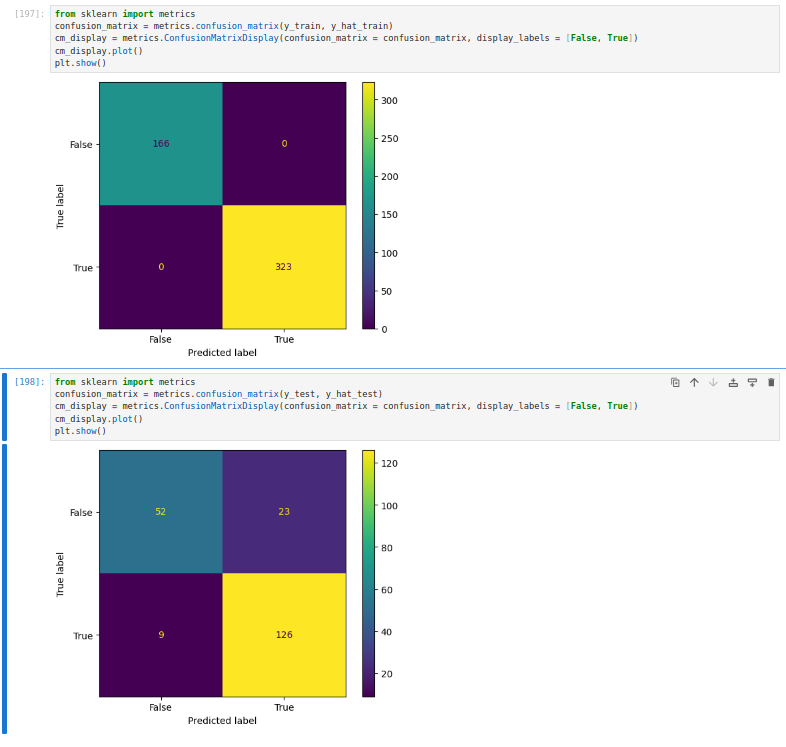
\includegraphics[height=3in]{Ex6/Breast_Cancer/matrix_conf_300.png}
\vspace{10pt}

\end{center}

\begin{center}

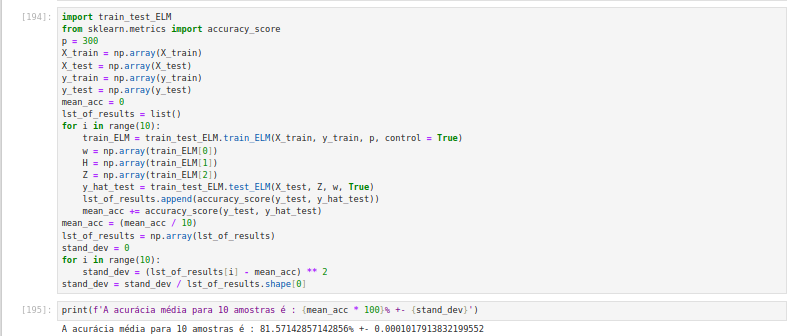
\includegraphics[height=3in]{Ex6/Breast_Cancer/acc_300.png}
\vspace{10pt}

\end{center}

Portanto, observando as matrizes de confusão e as acurácias médias, é possível afirmar que o modelo, ao usar 300 neuronios na camada intermediária é 1 modelo com overfitting. A acurácia permanece a mesma com 30, 50 e 100 neurônios. Para reduzir o custo computacional, considerando-se que eles contém uma mesma acurácia, o modelo com 30 neuronios na camada intermediária generaliza melhor.




\subsection{Hearth Disease}
O dataset Hearth Disease foi utilizado.

\begin{center}

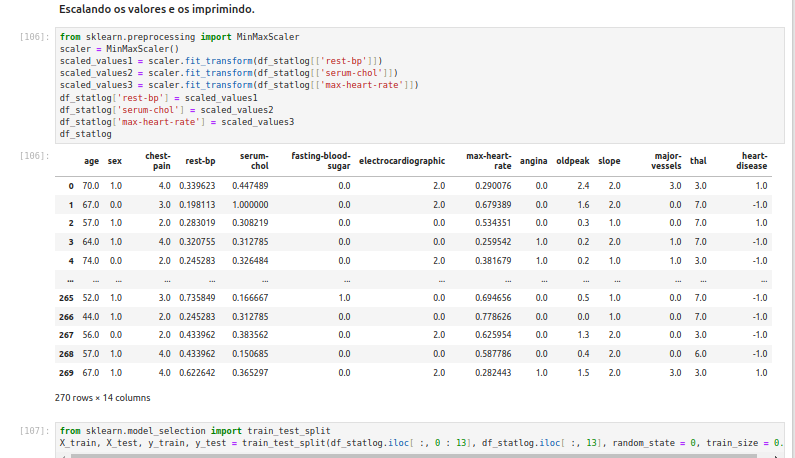
\includegraphics[height=2in]{Ex6/Hearth_Disease/data_health.png}

\end{center}

\vspace{5pt}
Inicialmente foi utilizado uma ELM com 5 neurônios na camada intermediária. Com apenas 5 neurônios na camada intermediária, é possível concluir que o modelo obteve um alto erro para os dados tanto de treino quanto de teste, os erros foram bastante altos e podemos considerar isso como um underfitting. A matriz de confusão e o gráfico de separação estão plotados abaixo :

\begin{center}

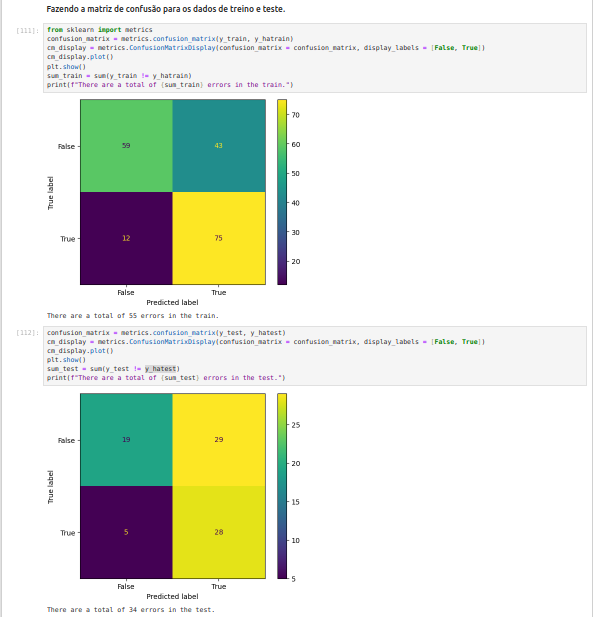
\includegraphics[height=3in]{Ex6/Hearth_Disease/conf_matrix_health_5.png}
\vspace{10pt}

\end{center}

\begin{center}

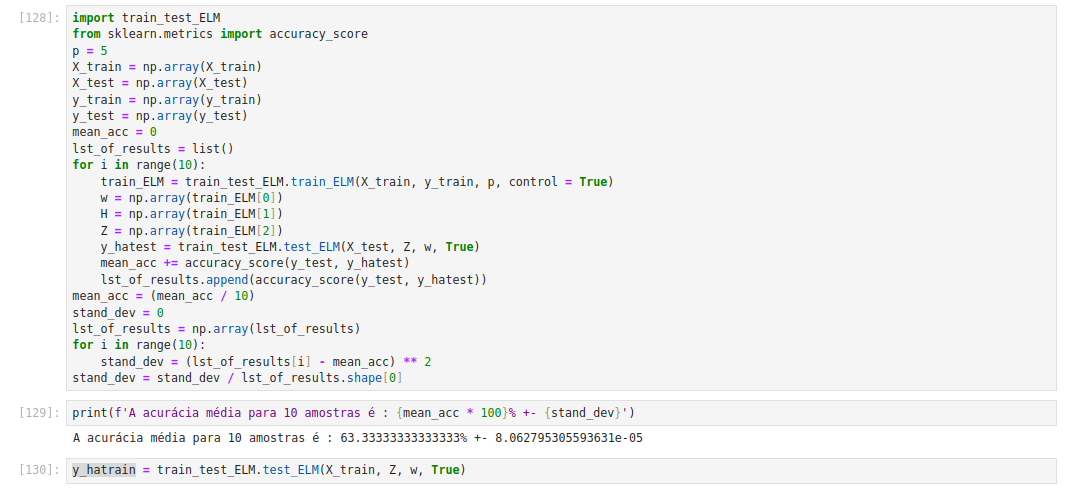
\includegraphics[height=3in]{Ex6/Hearth_Disease/acc_5.png}
\vspace{10pt}

\end{center}

\vspace{5pt}
Utilizando com 10 neuronios obtemos os resultados : 

\begin{center}

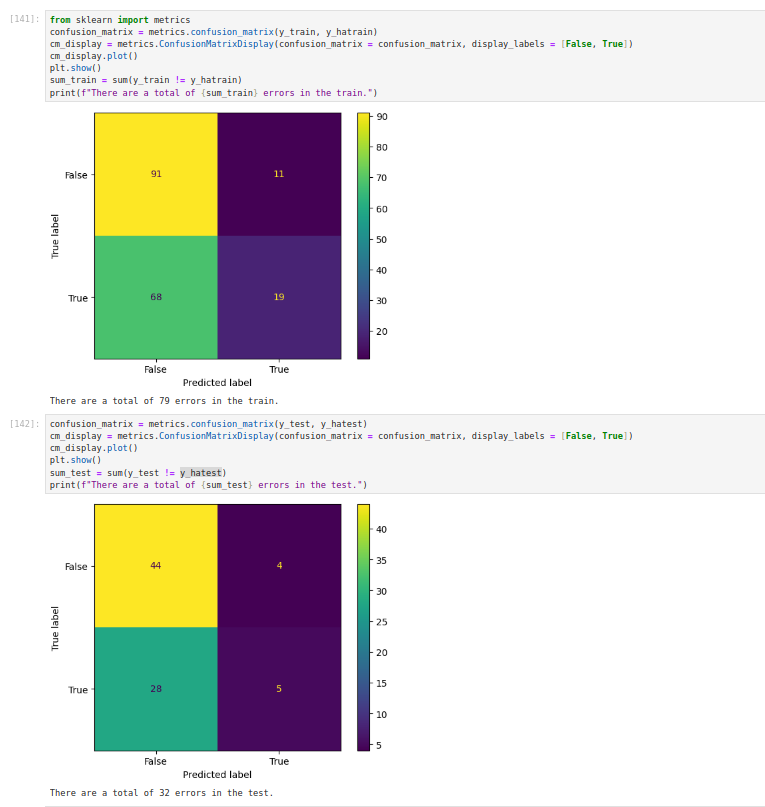
\includegraphics[height=3in]{Ex6/Hearth_Disease/conf_matrix_health_10.png}
\vspace{10pt}

\end{center}

\begin{center}

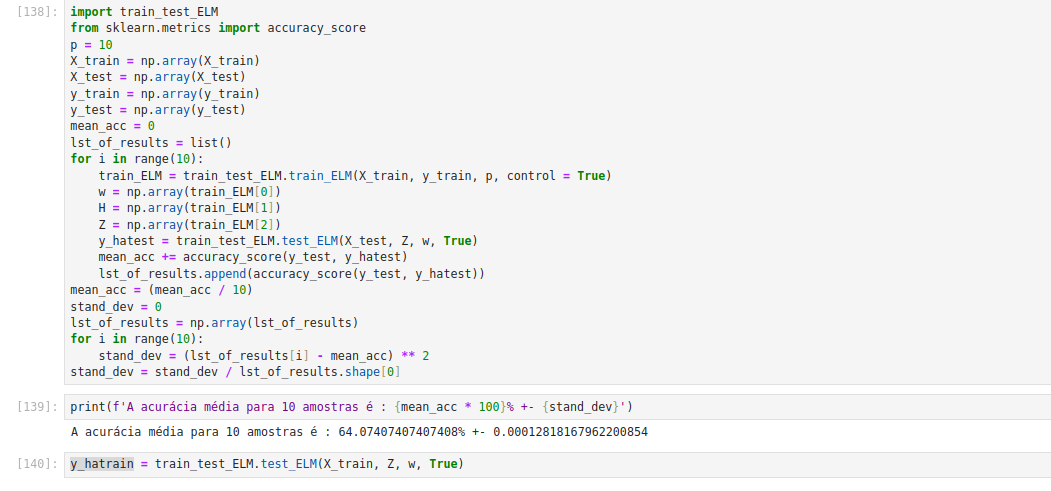
\includegraphics[height=3in]{Ex6/Hearth_Disease/acc_10.png}
\vspace{10pt}

\end{center}

\vspace{5pt}
Utilizando com 30 neuronios obtemos os resultados : 

\begin{center}

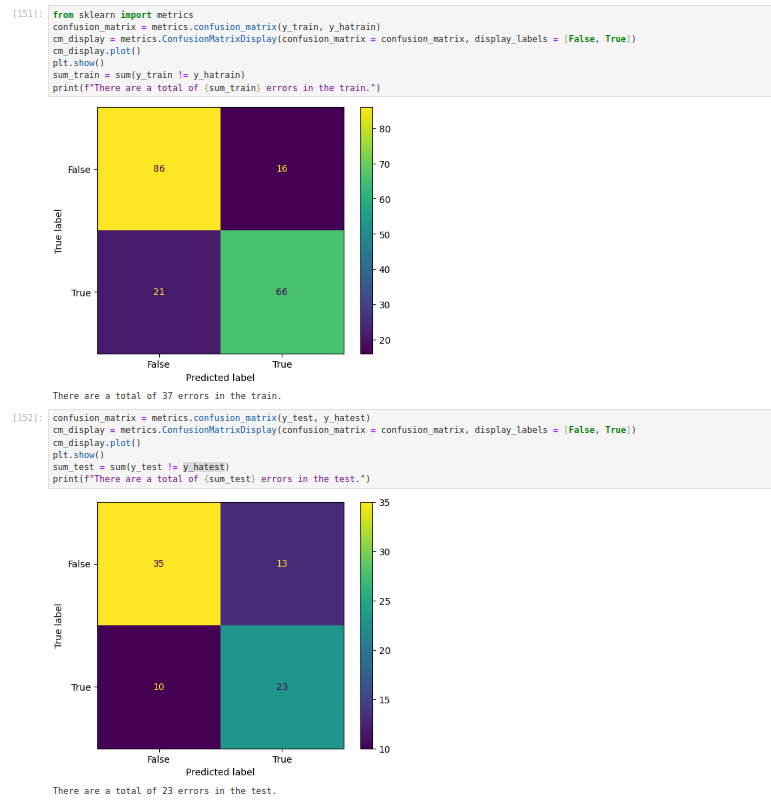
\includegraphics[height=3in]{Ex6/Hearth_Disease/conf_matrix_health_30.png}
\vspace{10pt}

\end{center}

\begin{center}

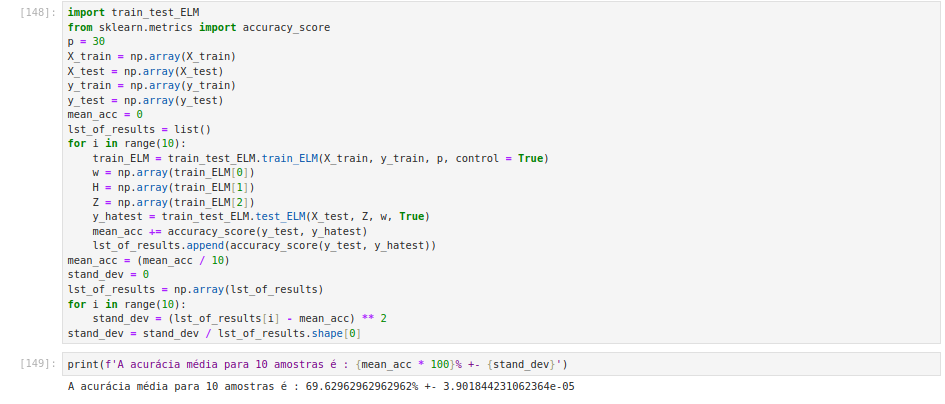
\includegraphics[height=3in]{Ex6/Hearth_Disease/acc_30.png}
\vspace{10pt}

\end{center}

\vspace{5pt}
Utilizando com 50 neuronios obtemos os resultados : 

\begin{center}

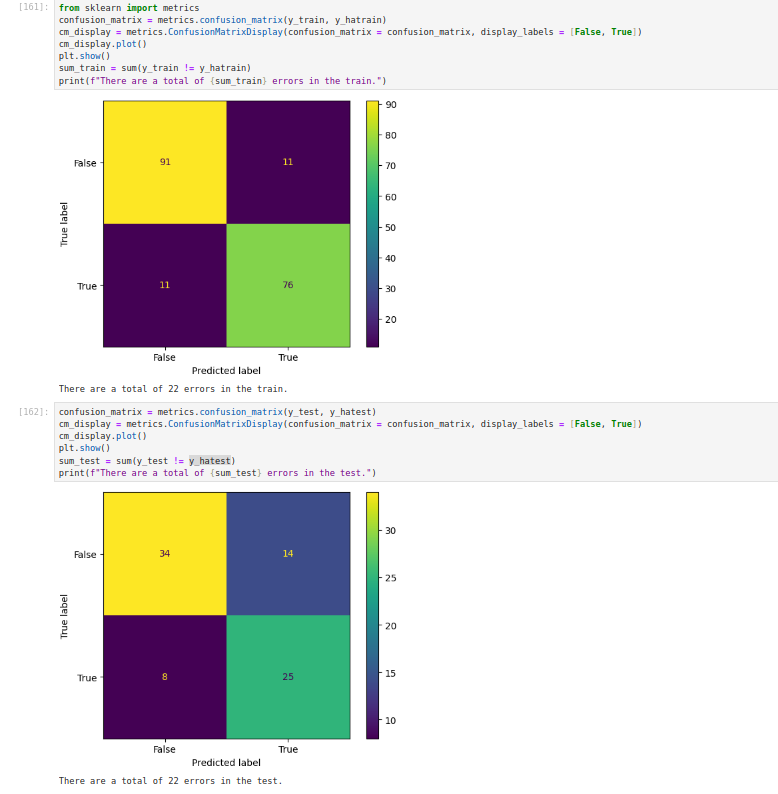
\includegraphics[height=3in]{Ex6/Hearth_Disease/conf_mat_50.png}
\vspace{10pt}

\end{center}

\begin{center}

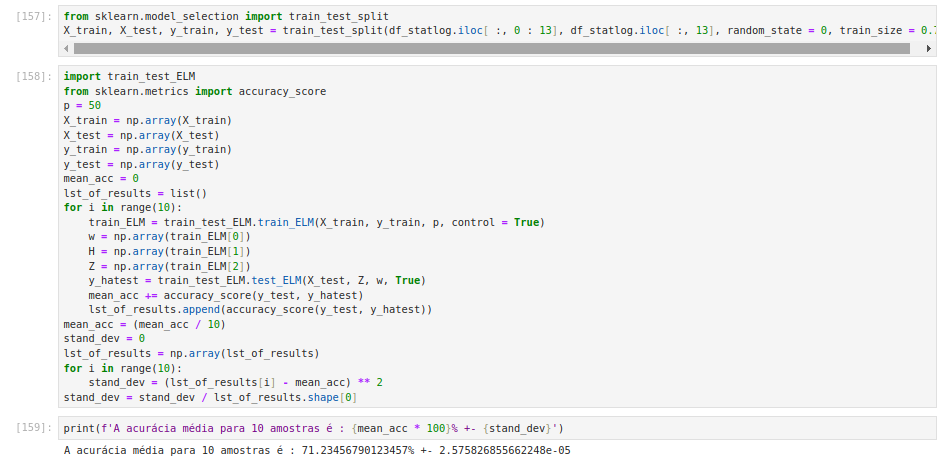
\includegraphics[height=3in]{Ex6/Hearth_Disease/acc_50.png}
\vspace{10pt}

\end{center}



\vspace{5pt}
Utilizando com 100 neuronios obtemos os resultados : 

\begin{center}

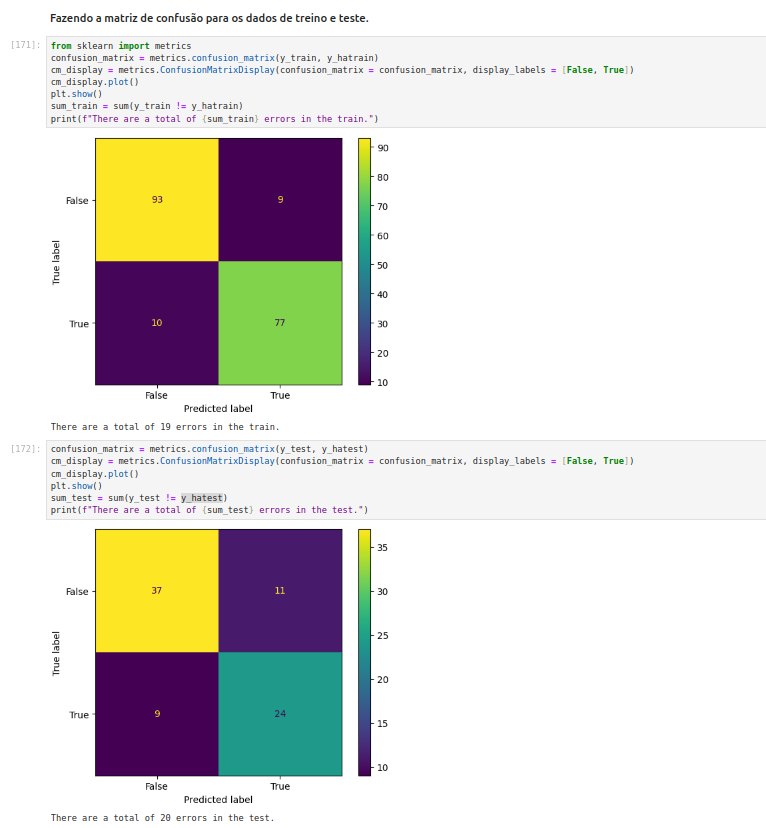
\includegraphics[height=3in]{Ex6/Hearth_Disease/conf_mat_100.png}
\vspace{10pt}

\end{center}

\begin{center}

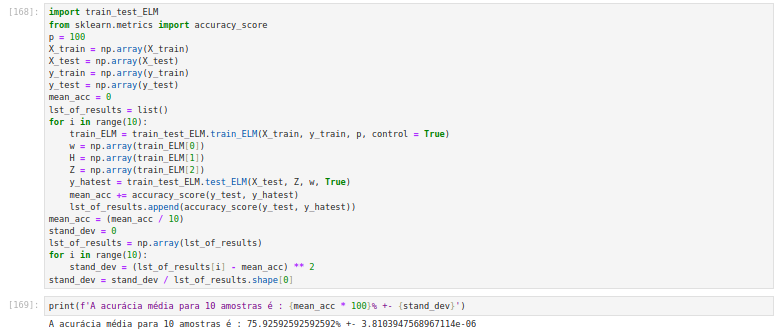
\includegraphics[height=3in]{Ex6/Hearth_Disease/acc_100.png}
\vspace{10pt}

\end{center}



\vspace{5pt}
Utilizando com 300 neuronios obtemos os resultados : 

\begin{center}

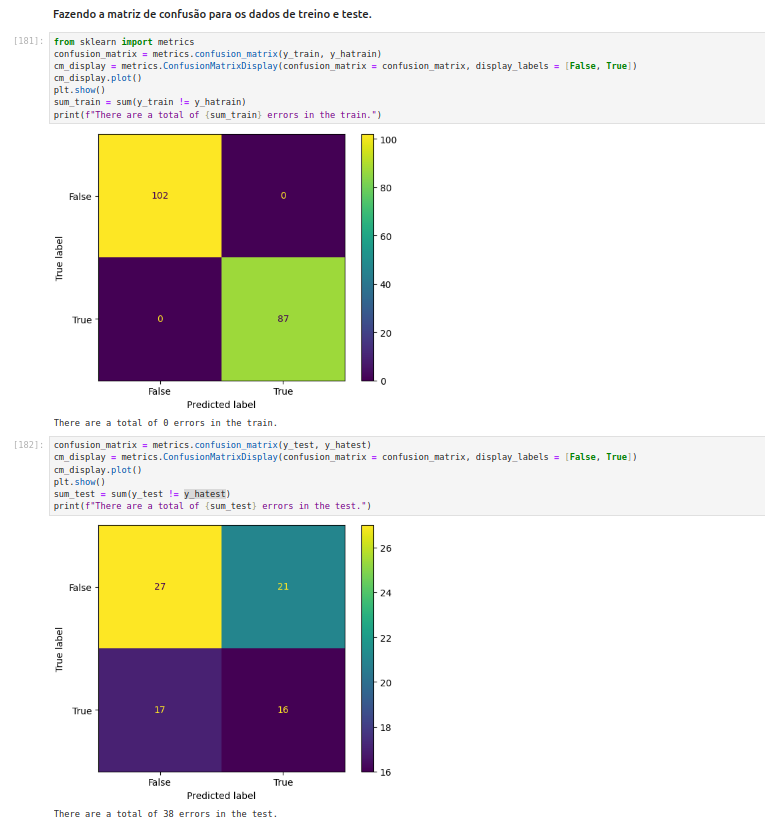
\includegraphics[height=3in]{Ex6/Hearth_Disease/conf_mat_300.png}
\vspace{10pt}

\end{center}

\begin{center}

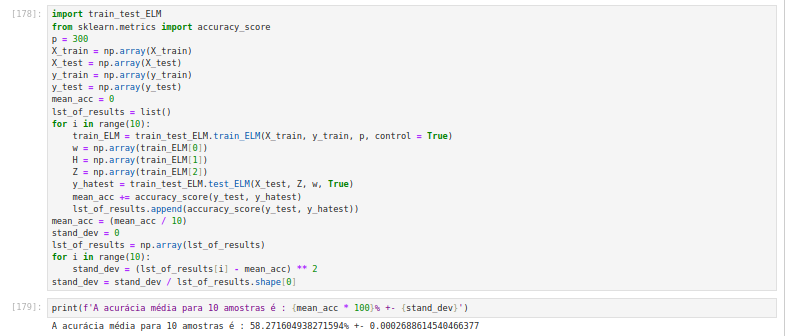
\includegraphics[height=3in]{Ex6/Hearth_Disease/acc_300.png}
\vspace{10pt}

\end{center}

Portanto, observando as matrizes de confusão e as acurácias médias, é possível afirmar que o modelo, ao usar 300 neuronios na camada intermediária é 1 modelo com overfitting. Portanto, o modelo com a melhor generalização é o modelo que contém 100 neurônios na camada intermediária.
\vspace{10pt}

Os dois exemplos de redes ELM mostram que os resultados da acurácia aumentam conforme o número de neuronios da camada intermediária. No entanto, há um certo limite de neurônios que fazem com que o modelo seja um overfitting. A ideia é ajustar corretamente o hyperparametro p para a boa generalização do modelo.



\subsection{Perceptron}
Agora, iremos utilizar o perceptron simples sobre os mesmos conjunto de dados, e avaliar a performance dele através da acurácia e a matriz de confusão. A função de treino do perceptron simples é mostrada abaixo : 
\begin{center}

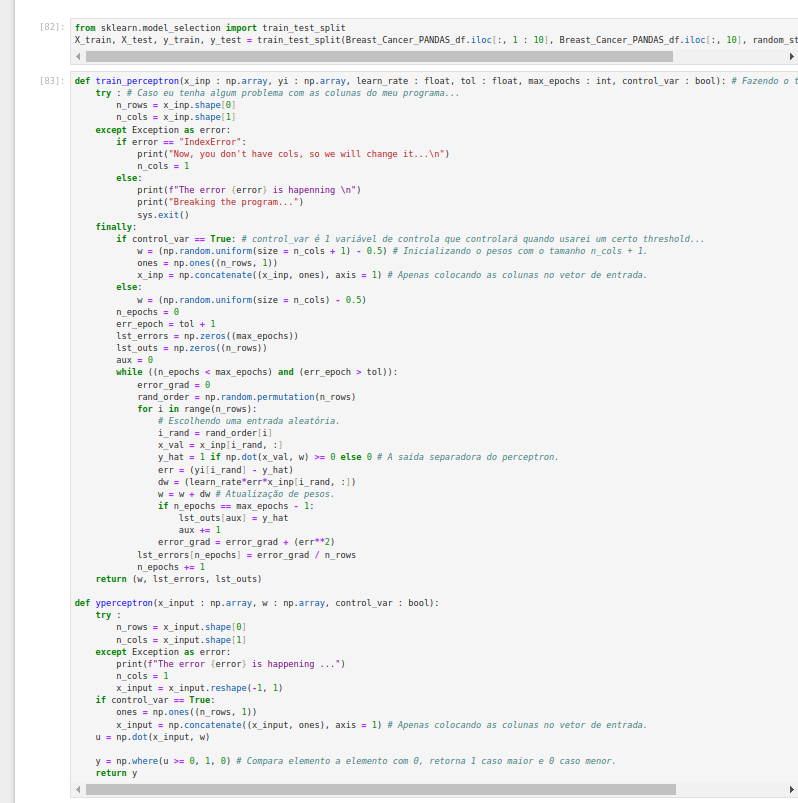
\includegraphics[height=3in]{Ex6/perceptron/train_perceptron.png}
\vspace{10pt}

\end{center}


Os restultados do perceptron tanto para o Breast Cancer quanto para o Hearth Disease estão plotados abaixo : 

\vspace{10pt}

Breast Cancer : 

\begin{center}

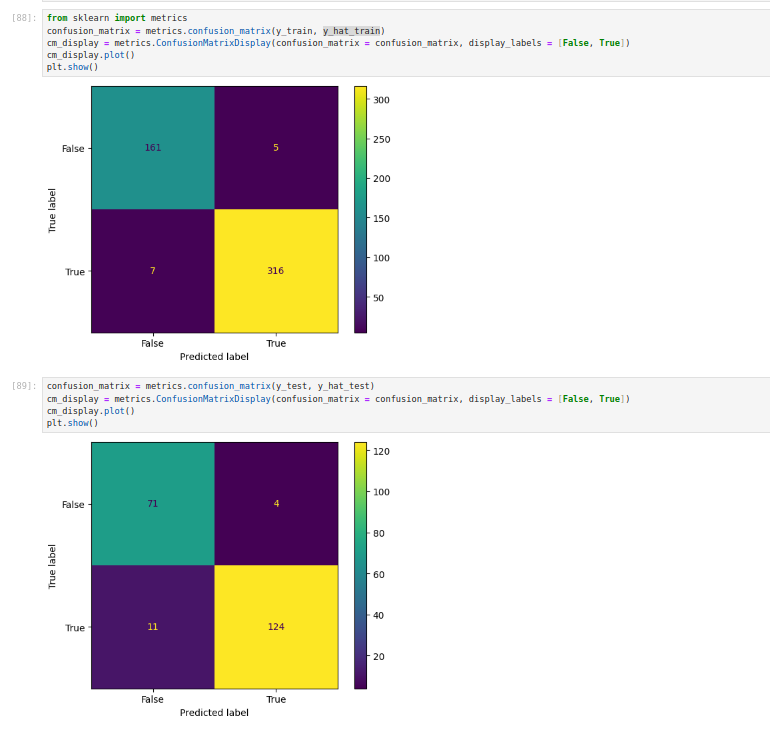
\includegraphics[height=3in]{Ex6/perceptron/conf_matrix_Breast.png}
\vspace{10pt}

\end{center}

\begin{center}
    
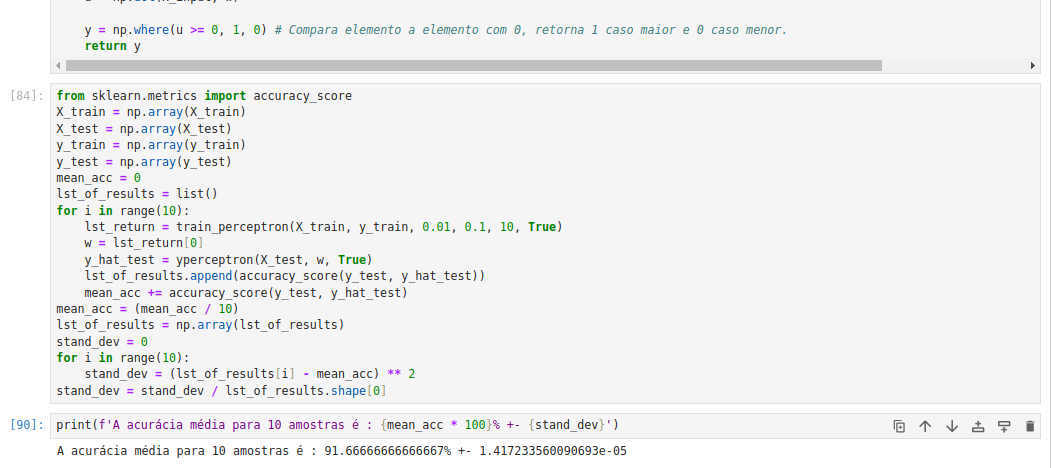
\includegraphics[height=3in]{Ex6/perceptron/acc_Breast_Cancer.png}
\vspace{10pt}

\end{center}

\vspace{10pt}

Hearth Disease : 

\begin{center}

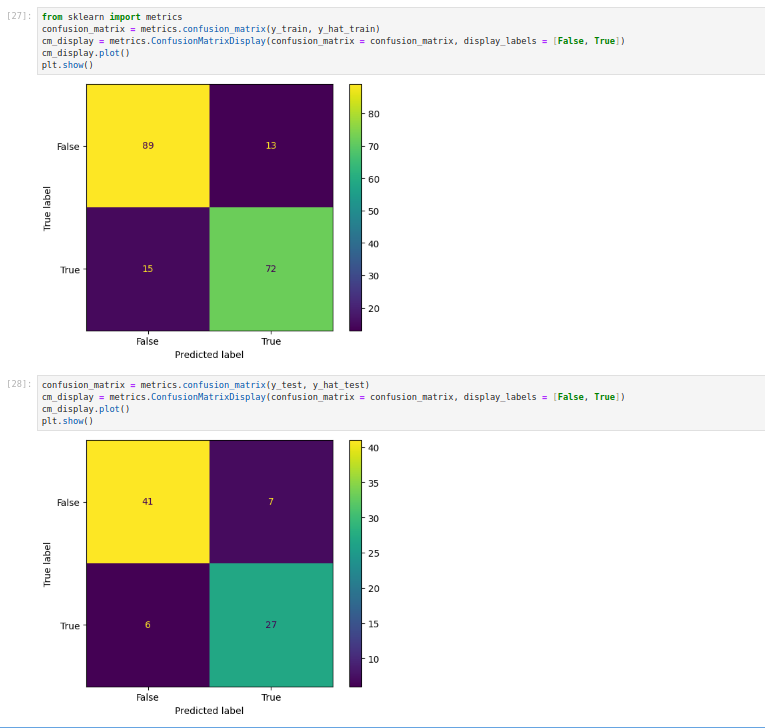
\includegraphics[height=3in]{Ex6/perceptron/conf_matrix_hearth.png}
\vspace{10pt}

\end{center}

\begin{center}
    
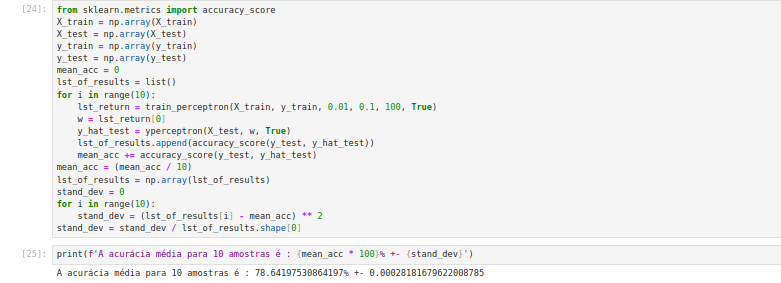
\includegraphics[height=3in]{Ex6/perceptron/acc_hearth.png}
\vspace{10pt}

\end{center}

Após analisar tanto a acurácia do perceptron simples quanto a acurácia das redes ELM é possível concluir que o dataset Hearth Disease é um dataset com uma correlação mais complexa entre as variáveis, pois a acurácia é baixa mesmo variando diversas vezes os parâmetros da rede de modo a tentar melhorar a acurácia.

\end{document}
